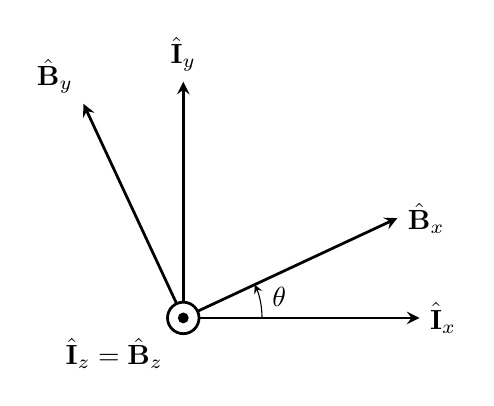
\begin{tikzpicture}[>=stealth, line width=1pt, scale=2.5]
    \def\thetaAngle{25}
    \def\axisLen{1.2}

    % Inertial frame
    \draw[->] (0,0) -- (\axisLen,0) node[right] {$\hat{\mathbf{I}}_x$};
    \draw[->] (0,0) -- (0,\axisLen) node[above] {$\hat{\mathbf{I}}_y$};

    % Body frame rotated by theta Angle
    \draw[->] (0,0) -- (\thetaAngle:\axisLen) node[right] {$\hat{\mathbf{B}}_x$};
    \draw[->] (0,0) -- (90+\thetaAngle:\axisLen) node[above left] {$\hat{\mathbf{B}}_y$};

    % Common z-axis, pointing out of the page
    \filldraw[fill=white, draw=black] (0,0) circle (0.08);
    \filldraw[black] (0,0) circle (0.02);
    \node[anchor=north east] at (-0.05,-0.05) {$\hat{\mathbf{I}}_z = \hat{\mathbf{B}}_z$};

    % Rotation angle
    \draw[->, thin] (0.4,0) arc (0:\thetaAngle:0.4);
    \node at ({\thetaAngle/2}:0.5) {$\theta$};
\end{tikzpicture}
